\documentclass[10pt]{article}

\usepackage[letterpaper,margin=0.72in,headheight=15pt]{geometry}
\usepackage{amsmath,amssymb}
\usepackage{booktabs,longtable,tabularx,array,multirow}
\usepackage{graphicx,float,caption,subcaption}
\usepackage{adjustbox}
\usepackage[dvipsnames,table]{xcolor}
\usepackage{tikz}
\usetikzlibrary{arrows.meta,positioning,shapes.geometric,fit,calc}
\usepackage{enumitem}
\usepackage{fancyhdr}
\usepackage{titlesec}
\usepackage{microtype}
\usepackage[hidelinks]{hyperref}

\definecolor{navy}{HTML}{17365D}
\definecolor{blue}{HTML}{3D6FA8}
\definecolor{lightblue}{HTML}{EAF1F8}
\definecolor{green}{HTML}{2E7D54}
\definecolor{lightgreen}{HTML}{EAF5EF}
\definecolor{orange}{HTML}{C66A05}
\definecolor{lightorange}{HTML}{FFF1DF}
\definecolor{red}{HTML}{A52A2A}
\definecolor{lightred}{HTML}{F9E9E9}
\definecolor{grey}{HTML}{555555}
\definecolor{lightgrey}{HTML}{F2F4F6}

\newcommand{\method}[1]{\textsf{#1}}
\newcommand{\yes}{\textcolor{green}{Yes}}
\newcommand{\no}{\textcolor{red}{No}}
\newcommand{\project}{\textcolor{orange}{Project ablation}}
\newcommand{\published}{\textcolor{green}{Published component}}
\newcommand{\warningbox}[1]{%
  \begin{center}
  \fcolorbox{red}{lightred}{\begin{minipage}{0.94\linewidth}\textbf{Critical limitation.} #1\end{minipage}}
  \end{center}}
\newcommand{\decisionbox}[1]{%
  \begin{center}
  \fcolorbox{navy}{lightblue}{\begin{minipage}{0.94\linewidth}\textbf{Current decision.} #1\end{minipage}}
  \end{center}}

\pagestyle{fancy}
\fancyhf{}
\lhead{RR-HRV Cascade Audit}
\rhead{Current-state addendum}
\cfoot{\thepage}
\titleformat{\section}{\Large\bfseries\color{navy}}{\thesection}{0.6em}{}
\titleformat{\subsection}{\large\bfseries\color{navy}}{\thesubsection}{0.6em}{}
\setlist{nosep,leftmargin=1.4em}
\setlength{\parindent}{0pt}
\setlength{\parskip}{0.42em}
\graphicspath{{../outputs/interval_consistent_fusion_all48_v1/}{../outputs/unsw_neurokit_zhai_fusion_all48_v1/}}

\begin{document}
\hypersetup{pageanchor=false}

\begin{titlepage}
\centering
\vspace*{1.25in}
{\Huge\bfseries\color{navy} RR-HRV Cascade\par}
\vspace{0.16in}
{\LARGE Complete Method Audit and Current Candidate Architecture\par}
\vspace{0.35in}
{\Large Current-state addendum to the R-peak detector audit\par}
\vfill
\begin{minipage}{0.82\linewidth}
\fcolorbox{navy}{lightblue}{\begin{minipage}{0.94\linewidth}
\textbf{Working candidate:} NeuroKit $\rightarrow$ Zhai $\rightarrow$ UNSW,
with same-source endpoints inside every RR interval. The candidate is retained
because it gives complete coverage and the best pooled full-coverage RR error
among the tested hierarchies. It is not yet a clinically validated timestamp
owner because adjacent RR intervals can still change detector source.
\end{minipage}}
\end{minipage}
\vfill
{\large August 7, 2026\par}
{\normalsize Working technical report - feature-extraction validation, not seizure validation\par}
\end{titlepage}

\hypersetup{pageanchor=true}
\pagenumbering{roman}
\tableofcontents
\clearpage
\pagenumbering{arabic}

\section{Scope and Evidence Boundary}

This addendum consolidates every R-peak, RR, and HRV method tested after the
original audit. The preceding report retains the detailed Pan--Tompkins,
NeuroKit, UNSW/Khamis, polarity, bundle-branch morphology, and five-record case
studies. This section adds the completed 48-record detector/fiducial/fusion
comparisons and the current implementation contract.

The local audit used all 48 records from the MIT--BIH Arrhythmia Database,
channel 0, sampled at 360 Hz. Expert \texttt{atr} beat annotations were matched
within $\pm75$ ms. One sample equals 2.778 ms. The database has arrhythmia and
beat annotations but no seizure-onset, preictal, ictal, or postictal labels.

\warningbox{All ``high HRV'' threshold tests in this report measure whether an
algorithm preserves an expert-derived feature excursion. They do not establish
that the excursion is a seizure. Seizure sensitivity, false alarms per hour,
and latency require patient seizure labels and a chronologically held-out test
set.}

\subsection{Published components versus project decisions}

\begin{table}[H]
\centering
\caption{Evidence status of the current pipeline.}
\begin{tabularx}{\linewidth}{>{\raggedright\arraybackslash}p{0.29\linewidth}
                              >{\raggedright\arraybackslash}p{0.21\linewidth}X}
\toprule
Component & Status & What the evidence actually supports \\
\midrule
UNSW primary QRS detector with an independent secondary detector & \published & Ho et al. support primary-detector RR calculation with secondary-detector reliability assessment. \\
qSQI/detector agreement & \published & Zhao and Zhang support detector agreement as signal-quality context, not as a calibrated probability of correctness. \\
Direct downstream HRV concordance & \published & Weinstein et al. show why detector F1 alone is insufficient and compare annotation-derived and detector-derived HRV using Lin CCC. \\
100-RR CSI, filtered ModCSI, and heart-rate slope & \published & Jeppesen et al. use these continuous measurements in a patient-specific seizure-detection system. \\
Zhai template-correlation fiducial & \published & Zhai et al. align a QRS template by normalized correlation; the local code is a documented reimplementation. \\
NeuroKit $\rightarrow$ Zhai $\rightarrow$ UNSW timestamp hierarchy & \project & No reviewed paper establishes this exact substitution order or its transition behavior. \\
Pure detector windows and whole-window priority & \project & These are local ablations designed to avoid mixing detector timestamps inside a 100-RR window. \\
\bottomrule
\end{tabularx}
\end{table}

\section{Every Method Tested and What It Taught Us}

\begin{longtable}{>{\raggedright\arraybackslash}p{0.17\linewidth}
                  >{\raggedright\arraybackslash}p{0.24\linewidth}
                  >{\raggedright\arraybackslash}p{0.26\linewidth}
                  >{\raggedright\arraybackslash}p{0.23\linewidth}}
\caption{Complete method inventory.}\label{tab:methods}\\
\toprule
Method & Exact role & Main result & Decision \\
\midrule
\endfirsthead
\toprule
Method & Exact role & Main result & Decision \\
\midrule
\endhead
\method{NeuroKit alone} & Gradient-based QRS-region detector followed by local positive-maximum localization. & Strong pooled detection, but record 113 produced T-wave double detections; records 207/108 exposed morphology and polarity sensitivity. & Retain as an independent candidate/context detector; not sufficient alone for unreviewed peri-ictal ECG. \\
\addlinespace
\method{Pan--Tompkins hard gate} & Kept a NeuroKit peak only when a Pan--Tompkins event occurred in a fixed timing gate. & Solved the specific record-113 T-wave pattern and removed record-231 intervening deflections, but exchanged false positives for false negatives and failed on changing morphology. & Rejected as a hard veto; retain only as historical/context ablation. \\
\addlinespace
\method{UNSW/Khamis} & Robust QRS-event detector; event existence and the original complete RR baseline. & Best pooled event-existence performance in the local 48-record comparison; its event timestamp is not always the anatomical R apex. & Retain as the always-available baseline and fallback event grid. \\
\addlinespace
\method{NeuroKit 250 ms} & Project modification of the detector separation rule. & Nearly identical sensitivity pattern to the unmodified 300-ms configuration; no meaningful advantage at the predeclared 50-ms association setting. & Do not replace the unmodified 300-ms baseline. \\
\addlinespace
\method{PhysioZoo/R-DECO localizers} & Local positive/negative extrema and envelope/correction challengers around a QRS proposal. & Pooled event matching could look good while wide, negative, or multi-lobed complexes moved to a different deflection. & Not selected as the final universal localizer. \\
\addlinespace
\method{Zhai reimplementation} & Bandpass, squared QRS envelope, dynamic windows, representative template, normalized cross-correlation fiducial. & Best conditional RR precision lane in the present audit; availability and full-window coverage were lower and missingness was non-random. & Retain as the best precision challenger and second interval fallback. \\
\addlinespace
\method{Old per-beat fusion} & Chose NeuroKit, else Zhai, else UNSW separately at each beat, then differenced the resulting beat sequence. & Good timing and RR error, but created mixed-source intervals and large errors at detector transitions. & Rejected as the current implementation. \\
\addlinespace
\method{UNSW-only RR with NK context} & Every RR used UNSW at both ends; NeuroKit supplied unique support, offsets, ambiguity, and qSQI. & Prevented timestamp-source switching and produced strong J1/J2 CCC, but retained higher RR MAE. & Retain as the conservative baseline. \\
\addlinespace
\method{Same-source-per-RR fusion} & Each RR independently uses NeuroKit at both ends, else Zhai at both ends, else UNSW at both ends. & Removed every mixed-endpoint RR and gave the best full-coverage pooled RR MAE, but adjacent RRs can still change source. & Current working candidate; transition-aware and not yet clinically locked. \\
\addlinespace
\method{Pure NK/Zhai windows} & Calculate HRV only from a fully contiguous detector-specific timestamp run. & Highest conditional HRV concordance; NeuroKit covered 71\% and Zhai 57\% of 100-RR windows. & Retain as parallel precision outputs; missing means unknown, never normal. \\
\addlinespace
\method{Whole-window priority} & Use a complete pure NeuroKit window, else pure Zhai window, else complete UNSW window. & Complete output and near-baseline threshold preservation; did not dominate UNSW on all metrics. & Retain as an offline challenger, not a silent replacement. \\
\bottomrule
\end{longtable}

\section{Prior Standalone and Fusion Results}

\begin{table}[H]
\centering
\caption{Earlier all-48 detector and fiducial comparison.}
\begin{tabular}{lrrr}
\toprule
Method & Beat/event $F_1$ & Mean timing error (ms) & RR MAE (ms) \\
\midrule
UNSW initial event stream & 0.997261 & 8.705 & 3.971 \\
NeuroKit 300-ms strict & 0.980334 & 3.574 & 3.307 \\
Zhai 2023 reimplementation & 0.985637 & 5.232 & 3.832 \\
Old per-beat NeuroKit--Zhai--UNSW fusion & 0.997070 & 3.009 & 3.382 \\
\bottomrule
\end{tabular}
\end{table}

The timing winner and RR winner need not be the same. A constant fiducial
offset cancels when adjacent timestamps use the same convention; changing
offsets or source transitions create false RR variability. Therefore, the next
audit evaluated RR error, successive-RR-change error, and the actual downstream
J1/J2 outputs rather than selecting a method from beat $F_1$ alone.

\section{Current Candidate: NeuroKit to Zhai to UNSW}

\subsection{Detailed architecture}

\begin{figure}[H]
\centering
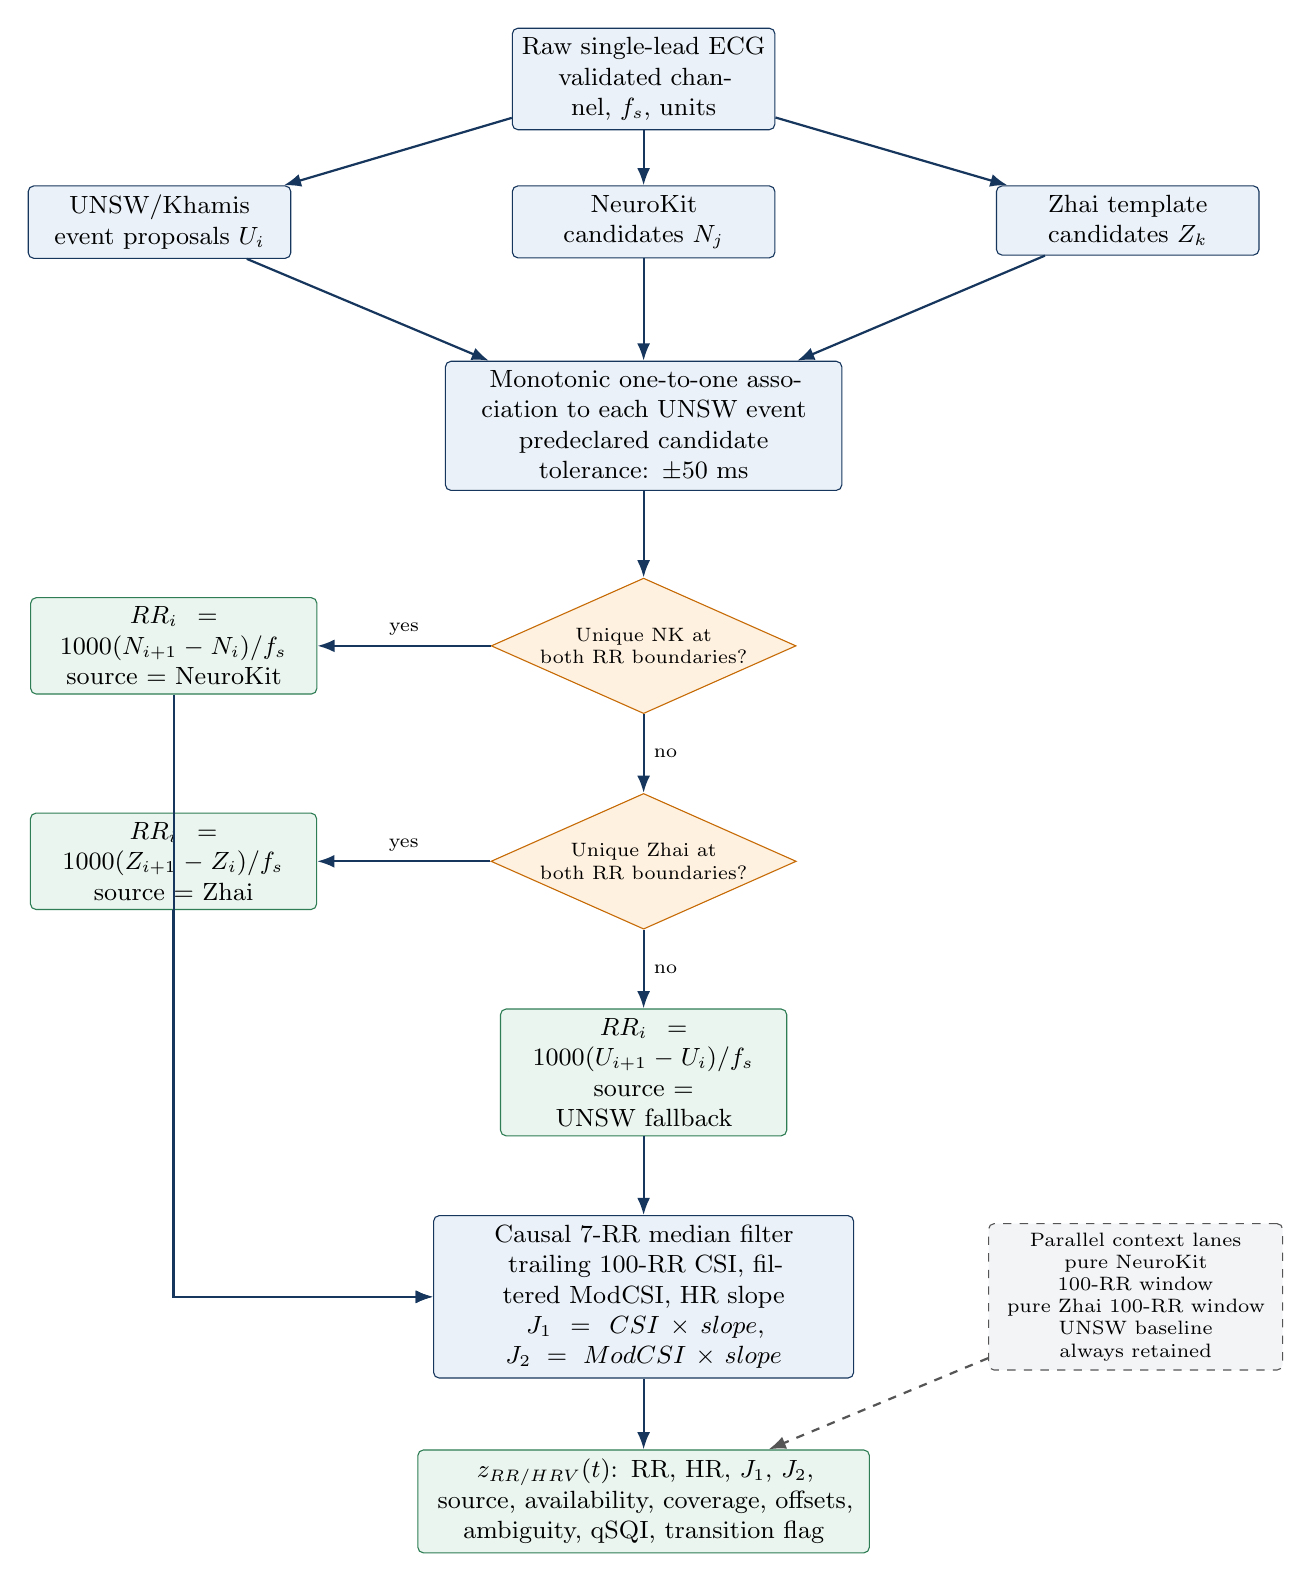
\begin{tikzpicture}[
  node distance=7mm and 8mm,
  box/.style={draw=navy,rounded corners=2pt,fill=lightblue,align=center,
              minimum height=8mm,text width=31mm,font=\small},
  decision/.style={draw=orange,diamond,aspect=2.25,fill=lightorange,
                   align=center,font=\scriptsize,inner sep=1pt},
  outputbox/.style={draw=green,rounded corners=2pt,fill=lightgreen,align=center,
              minimum height=8mm,text width=34mm,font=\small},
  context/.style={draw=grey,dashed,rounded corners=2pt,fill=lightgrey,
                  align=center,text width=35mm,font=\scriptsize},
  arrow/.style={-{Latex[length=2.2mm]},thick,draw=navy}
]
\node[box] (ecg) {Raw single-lead ECG\\validated channel, $f_s$, units};
\node[box,below left=of ecg,xshift=-20mm] (unsw) {UNSW/Khamis\\event proposals $U_i$};
\node[box,below=of ecg] (nk) {NeuroKit\\candidates $N_j$};
\node[box,below right=of ecg,xshift=20mm] (zhai) {Zhai template\\candidates $Z_k$};
\node[box,below=13mm of nk,text width=48mm] (assoc) {Monotonic one-to-one association to each UNSW event\\predeclared candidate tolerance: $\pm50$ ms};
\node[decision,below=11mm of assoc] (dnk) {Unique NK at\\both RR boundaries?};
\node[decision,below=10mm of dnk] (dz) {Unique Zhai at\\both RR boundaries?};
\node[outputbox,left=22mm of dnk] (rrnk) {$RR_i=1000(N_{i+1}-N_i)/f_s$\\source = NeuroKit};
\node[outputbox,left=22mm of dz] (rrz) {$RR_i=1000(Z_{i+1}-Z_i)/f_s$\\source = Zhai};
\node[outputbox,below=10mm of dz] (rru) {$RR_i=1000(U_{i+1}-U_i)/f_s$\\source = UNSW fallback};
\node[box,below=10mm of rru,text width=51mm] (features) {Causal 7-RR median filter\\trailing 100-RR CSI, filtered ModCSI, HR slope\\$J_1=CSI\times slope$, $J_2=ModCSI\times slope$};
\node[outputbox,below=9mm of features,text width=55mm] (output) {$z_{RR/HRV}(t)$: RR, HR, $J_1$, $J_2$, source, availability, coverage, offsets, ambiguity, qSQI, transition flag};
\node[context,right=17mm of features] (pure) {Parallel context lanes\\pure NeuroKit 100-RR window\\pure Zhai 100-RR window\\UNSW baseline always retained};

\draw[arrow] (ecg) -- (unsw);
\draw[arrow] (ecg) -- (nk);
\draw[arrow] (ecg) -- (zhai);
\draw[arrow] (unsw) -- (assoc);
\draw[arrow] (nk) -- (assoc);
\draw[arrow] (zhai) -- (assoc);
\draw[arrow] (assoc) -- (dnk);
\draw[arrow] (dnk) -- node[above,font=\scriptsize]{yes} (rrnk);
\draw[arrow] (dnk) -- node[right,font=\scriptsize]{no} (dz);
\draw[arrow] (dz) -- node[above,font=\scriptsize]{yes} (rrz);
\draw[arrow] (dz) -- node[right,font=\scriptsize]{no} (rru);
\draw[arrow] (rrnk.south) |- (features.west);
\draw[arrow] (rrz.south) |- (features.west);
\draw[arrow] (rru) -- (features);
\draw[arrow] (features) -- (output);
\draw[arrow,dashed,draw=grey] (pure) -- (output);
\end{tikzpicture}
\caption{Current working architecture. UNSW owns the event grid. Every selected RR has
same-source endpoints. Reliability remains an output, not a hard veto.}
\end{figure}

\subsection{Exact interval rule}

For UNSW-indexed heartbeat $i$ and $i+1$,
\begin{equation}
RR_i=
\begin{cases}
1000(N_{i+1}-N_i)/f_s,
&\text{if both unique NeuroKit candidates exist},\\[3pt]
1000(Z_{i+1}-Z_i)/f_s,
&\text{otherwise, if both unique Zhai candidates exist},\\[3pt]
1000(U_{i+1}-U_i)/f_s,
&\text{otherwise}.
\end{cases}
\end{equation}

This prevents $N_{i+1}-U_i$ and $U_{i+1}-N_i$. It does not produce one global
timestamp sequence because $RR_i$ can use NeuroKit while $RR_{i+1}$ uses UNSW.
The common heartbeat then has $N_{i+1}$ in one interval and $U_{i+1}$ in the
next. The implementation therefore exports the source and a transition flag
for every interval.

\subsection{HRV calculations}

For each trailing 100-RR window, the implementation calculates Poincare axes
$SD1$ and $SD2$, then
\begin{align}
CSI_{100} &= \frac{SD2_{raw}}{SD1_{raw}},\\
ModCSI^{(7)}_{100} &= \frac{(4SD2_{filtered})^2}{4SD1_{filtered}},\\
Slope_{100} &= \left|\frac{\sum_j(t_j-\bar{t})(HR_j-\overline{HR})}
                         {\sum_j(t_j-\bar{t})^2}\right|,\\
J_1 &= CSI_{100}\,Slope_{100},\\
J_2 &= ModCSI^{(7)}_{100}\,Slope_{100}.
\end{align}

The seven-RR median filter is causal. A pure detector-specific 100-RR window
requires 107 consecutive candidate events: 101 events define 100 RR intervals,
and six earlier intervals provide full median-filter history.

\section{Complete Primary-Setting Results}

The primary comparison was declared as the unmodified NeuroKit 300-ms strict
configuration with a $\pm50$-ms candidate association. RR sensitivity was also
tested at 75, 100, and 150 ms and with the project NeuroKit 250-ms variant.

\begin{table}[H]
\centering
\caption{Complete all-48 comparison. q95 $F_1$ is same-threshold feature
preservation, not seizure classification.}
\begin{adjustbox}{max width=\linewidth}
\begin{tabular}{lrrrrrrr}
\toprule
Method & RR avail. & RR MAE & $\Delta RR$ MAE & HRV cov. & J1 CCC & J2 CCC & q95 $F_1$ J1/J2 \\
 & (\%) & (ms) & (ms) & (\%) & & & \\
\midrule
UNSW baseline & 100.0 & 3.971 & 7.325 & 100.0 & 0.990377 & 0.993876 & 0.860/0.860 \\
Old per-beat fusion & 100.0 & 3.416 & 6.627 & 100.0 & 0.990785 & 0.994326 & 0.863/0.846 \\
NK then UNSW per RR & 100.0 & 3.185 & 6.163 & 100.0 & 0.990786 & 0.994337 & 0.863/0.849 \\
Zhai then UNSW per RR & 100.0 & 3.523 & 6.776 & 100.0 & 0.990387 & 0.994169 & 0.853/0.857 \\
\rowcolor{lightblue}NK then Zhai then UNSW per RR & 100.0 & \textbf{3.182} & \textbf{6.166} & 100.0 & 0.990778 & \textbf{0.994390} & 0.862/0.846 \\
Pure NeuroKit lane & 95.3 & 2.967 & 5.675 & 71.0 & \textbf{0.999633} & 0.996874 & 0.942/0.939$^{*}$ \\
Pure Zhai lane & 93.2 & \textbf{2.706} & \textbf{5.161} & 57.3 & 0.999340 & \textbf{0.998084} & \textbf{0.948/0.942}$^{*}$ \\
Whole-window NK/Zhai/UNSW priority & -- & -- & -- & 100.0 & 0.990682 & 0.993677 & 0.863/0.860 \\
\bottomrule
\end{tabular}
\end{adjustbox}
\end{table}

\noindent $^{*}$Pure-lane $F_1$ is conditional on available windows. If missing windows are
treated as missed expert-high events, q95 hard-veto $F_1$ falls to 0.718/0.693
for NeuroKit and 0.586/0.539 for Zhai. Missing means unknown, not normal.

\begin{figure}[H]
\centering
\includegraphics[width=0.98\linewidth]{rr_and_successive_change_comparison.png}
\caption{RR and successive-RR-change error. Pure lanes have lower error but
reduced availability. The combined hierarchy is the best full-coverage RR
method among the tested interval hierarchies.}
\end{figure}

\begin{figure}[H]
\centering
\includegraphics[width=0.98\linewidth]{hrv_method_concordance.png}
\caption{Direct downstream J1/J2 concordance with expert-derived features over
104,450 paired 100-RR windows. Pure-lane bars are conditional subsets and must
be interpreted with their displayed coverage.}
\end{figure}

\section{The Remaining Source-Transition Problem}

\begin{table}[H]
\centering
\caption{Error inside and between detector-source regimes.}
\begin{tabular}{lrrrr}
\toprule
Method & Mixed-endpoint & Source & Same-source & Transition \\
 & RRs & transitions & $\Delta RR$ MAE & $\Delta RR$ MAE \\
\midrule
Old per-beat fusion & 2,843 & 4,157 & 5.617 ms & 36.491 ms \\
NK then UNSW per RR & 0 & 2,051 & 5.902 ms & 21.892 ms \\
Zhai then UNSW per RR & 0 & 5,274 & 6.159 ms & 19.809 ms \\
NK then Zhai then UNSW per RR & 0 & 2,197 & 5.868 ms & 23.155 ms \\
\bottomrule
\end{tabular}
\end{table}

\begin{figure}[H]
\centering
\includegraphics[width=0.92\linewidth]{interval_source_transition_change_error.png}
\caption{The same-source-per-RR rule removes mixed endpoints but leaves a
measurable transition penalty between adjacent RRs.}
\end{figure}

Adding Zhai after NeuroKit changes pooled RR MAE by only 0.0029 ms relative to
the simpler NeuroKit--UNSW interval rule, while transition error increases and
q95 J2 $F_1$ decreases. This does not justify discarding the combined hierarchy,
because it still supplies complete coverage and the lowest full-coverage RR
MAE. It does justify retaining the simpler hierarchy as a required component
ablation and testing the untested reverse order, Zhai $\rightarrow$ NeuroKit
$\rightarrow$ UNSW, before permanently locking the priority.

\warningbox{The reverse Zhai-first hierarchy has not yet been benchmarked.
Pure Zhai's conditional advantage does not prove that Zhai should own the first
priority in a complete hierarchy. That ordering must be tested, not assumed.}

\section{Threshold Preservation and Coverage}

The q90/q95/q99 experiments ask whether a detector-derived feature crosses the
same per-record high threshold as the expert-derived feature. They are
measurement-fidelity stress tests. They are not the phase-3 seizure threshold
and are not trained classifiers.

\begin{figure}[H]
\centering
\includegraphics[width=0.98\linewidth]{threshold_method_comparison.png}
\caption{Same-threshold $F_1$ conditional on each method's available windows.
The pure lanes look strongest conditionally, but omit many expert-high windows.}
\end{figure}

At q95, pure NeuroKit retained 61.4\%/58.6\% of expert-high J1/J2 windows;
pure Zhai retained only 44.7\%/40.1\%. Therefore, low coverage is acceptable
only as an intentional abstention: an unavailable output must remain unknown,
must be passed to the final fusion as a missingness/availability field, and
must never be interpreted as non-seizure.

\section{Record-Level Generalization and Failure Cases}

The combined hierarchy improved RR MAE in 33 of 48 records and worsened it in
15. Mean paired record change was -0.836 ms and median change was -0.573 ms. An
exploratory Wilcoxon signed-rank test gave $p=0.00037$, while a 20,000-resample
record bootstrap interval for the mean change was [-1.80, +0.24] ms. The
bootstrap includes zero because a few records deteriorated severely. These are
development-set descriptions, not confirmatory clinical inference.

\begin{figure}[H]
\centering
\includegraphics[width=0.98\linewidth]{record_rr_mae_change_interval_hierarchy.png}
\caption{Record-level RR MAE change for the current combined hierarchy versus
UNSW. Green is improvement; red is deterioration.}
\end{figure}

\begin{table}[H]
\centering
\caption{Key records from the current hierarchy audit.}
\begin{tabularx}{\linewidth}{lrrrX}
\toprule
Record & UNSW MAE & Combined MAE & Change & Evidence-based interpretation \\
\midrule
108 & 8.379 & 9.220 & +0.840 & Mixed arrhythmia case remains worse under candidate substitution. \\
113 & 0.919 & 0.251 & -0.668 & The stable NeuroKit candidate lane corrects the earlier T-wave failure context. \\
200 & 6.757 & 22.223 & +15.467 & Catastrophic deterioration; header documents multiform PVCs and noise/artifact. \\
207 & 3.635 & 2.520 & -1.115 & Improves overall despite changing bundle-branch and ventricular morphology. \\
222 & 5.433 & 1.165 & -4.268 & Large improvement in the mixed arrhythmia/noise record. \\
231 & 1.525 & 1.235 & -0.290 & Modest improvement. \\
233 & 8.291 & 15.499 & +7.208 & Major deterioration; header documents multiform PVCs. \\
\bottomrule
\end{tabularx}
\end{table}

The record-200/233 association is consistent with morphology-dependent timing
failure but does not identify the mechanism of every error. A waveform-level
audit must test whether the candidate was moved to a different QRS lobe, whether
the QRS event itself was wrong, and whether detector agreement failed together.

\section{Tolerance and NeuroKit-Refractory Sensitivity}

\begin{figure}[H]
\centering
\includegraphics[width=0.98\linewidth]{tolerance_sensitivity.png}
\caption{Association-tolerance sensitivity. The 50-ms NeuroKit-300 setting was
declared before inspecting this result. Wider association windows generally
worsened RR and successive-change error.}
\end{figure}

For the combined NeuroKit--Zhai--UNSW hierarchy, RR/successive-change MAE was
3.182/6.166 ms at 50 ms, 3.364/6.528 ms at 75 ms, 3.395/6.585 ms at 100 ms,
and 3.892/7.568 ms at 150 ms. At 150 ms the successive-change error exceeded
the UNSW baseline. The NeuroKit 250-ms project experiment produced nearly the
same pattern and did not outperform the unmodified 300-ms configuration at the
predeclared 50-ms association.

\section{Final Working Implementation Contract}

\decisionbox{Keep NeuroKit $\rightarrow$ Zhai $\rightarrow$ UNSW as the
current complete-coverage candidate. Keep unchanged UNSW as a parallel baseline
and pure Zhai/NeuroKit as precision/context lanes. Do not call any unavailable
window normal, do not hard-veto detector disagreement, and do not claim seizure
validation.}

\subsection{Required inputs}

\begin{itemize}
\item one explicitly selected ECG channel, native sampling rate, physical units,
      duration, and missing-value audit;
\item UNSW/Khamis event samples $U_i$;
\item unmodified NeuroKit 300-ms candidate samples;
\item Zhai template-correlation candidate samples and correlation values;
\item monotonic one-to-one candidate association to the UNSW event grid at the
      locked 50-ms primary tolerance.
\end{itemize}

\subsection{Required per-event and per-RR fields}

\begin{table}[H]
\centering
\begin{tabularx}{\linewidth}{p{0.30\linewidth}X}
\toprule
Field group & Required content \\
\midrule
Event candidates & UNSW sample, unique NeuroKit sample or missing, unique Zhai sample or missing, both detector offsets from UNSW, association count, ambiguity. \\
Selected interval & start sample, end sample, RR ms, instantaneous HR, selected source, selection reason, same-source-endpoint assertion. \\
Transition context & previous RR source, source-transition flag, shared-boundary timestamp difference, ordering fallback. \\
Detector agreement & per-event support, per-RR support, extra secondary events, moving qSQI/agreement; never converted into an invented correctness probability. \\
HRV measurements & raw and causal-median RR, SD1, SD2, CSI, filtered ModCSI, elapsed-time HR slope, J1, J2, 100-RR window time and coverage. \\
Parallel lanes & unchanged UNSW J1/J2, pure NeuroKit J1/J2 when a full 107-event run exists, pure Zhai J1/J2 when a full run exists, and explicit availability masks. \\
\bottomrule
\end{tabularx}
\end{table}

\subsection{Assertions and failure behavior}

The implementation must assert:
\begin{enumerate}
\item every selected RR is positive and its two endpoints have the same source;
\item zero NeuroKit--UNSW or Zhai--UNSW mixed-endpoint RR intervals;
\item event indices and every detector-specific candidate sequence are monotonic;
\item the selected source and fallback reason are retained for every interval;
\item unavailable pure windows remain missing instead of being zero-filled;
\item no 100-RR window crosses a development/calibration/test split;
\item qSQI and detector disagreement remain context, not artifact labels or hard vetoes.
\end{enumerate}

\section{Next Validation Gate}

Before changing the timestamp owner or using this branch for a seizure alarm:
\begin{enumerate}
\item manually annotate representative clean, noisy, interictal, preictal,
      ictal, and postictal patient ECG, retaining QRS morphology;
\item split chronologically into development, baseline-threshold calibration,
      and untouched test periods;
\item lock the detector order, association tolerance, median filter, 100-RR
      features, and patient threshold before opening the test period;
\item report event $F_1$, timing error, RR MAE, successive-RR error, J1/J2 CCC,
      threshold crossing sensitivity/PPV/$F_1$, availability, and expert-high
      coverage;
\item report seizure sensitivity, false alarms per hour, and latency only after
      seizure labels are available;
\item test the reverse Zhai $\rightarrow$ NeuroKit $\rightarrow$ UNSW priority
      as a prespecified ablation, since pure Zhai was the conditional precision
      winner but a Zhai-first complete hierarchy has not been evaluated.
\end{enumerate}

\section{Reproducibility and Software Verification}

The current software includes 42 passing unit tests. The interval-consistent
test reproduces the exact transition example in which old per-beat fusion
creates 800/815 ms and the same-source-per-RR rule restores 800/800 ms. The
vectorized 100-RR calculation reproduces the previously audited calculation.
The all-48 benchmark stores record and pooled RR, HRV, threshold, coverage, and
decision tables under the versioned output directory
\path{feature_extraction/outputs/interval_consistent_fusion_all48_v1}.

\section*{Primary References}
\addcontentsline{toc}{section}{Primary References}

\begin{enumerate}
\item Goldberger AL et al. PhysioBank, PhysioToolkit, and PhysioNet.\
      \url{https://physionet.org/content/mitdb/1.0.0/}
\item Khamis H et al. Telehealth ECG QRS detection. IEEE Transactions on Biomedical Engineering, 2016.
\item Ho B et al. Automated RR Interval Detection and Quality Assessment in Telehealth. Computing in Cardiology, 2024.\
      \url{https://cinc.org/archives/2024/pdf/CinC2024-084.pdf}
\item Zhao Z, Zhang Y. SQI Quality Evaluation Mechanism of Single-Lead ECG Signal Based on Simple Heuristic Fusion and Fuzzy Comprehensive Evaluation. Frontiers in Physiology, 2018.\
      \url{https://pmc.ncbi.nlm.nih.gov/articles/PMC6011094/}
\item Weinstein A, Rodino J, Otero M. Effects of electrocardiogram QRS detection algorithms in heart rate variability metrics. Scientific Reports, 2026.\
      \url{https://doi.org/10.1038/s41598-026-49215-6}
\item Zhai X et al. QRS template matching and fiducial localization. Mathematical Biosciences and Engineering, 2023.\
      \url{https://doi.org/10.3934/mbe.2023848}
\item Jeppesen J et al. Detection of epileptic seizures with a modified heart rate variability algorithm based on Lorenz plot. Seizure, 2015.\
      \url{https://doi.org/10.1016/j.seizure.2014.11.004}
\item Jeppesen J et al. Seizure detection using wearable electrocardiogram connected to a smartphone: a phase 3 clinical validation study. EBioMedicine, 2025.\
      \url{https://pmc.ncbi.nlm.nih.gov/articles/PMC12516532/}
\end{enumerate}

\end{document}
